\documentclass[10pt]{article}
\usepackage[polish]{babel}
\usepackage[utf8]{inputenc}
\usepackage[T1]{fontenc}
\usepackage{amsmath}
\usepackage{amsfonts}
\usepackage{amssymb}
\usepackage[version=4]{mhchem}
\usepackage{stmaryrd}
\usepackage{graphicx}
\usepackage[export]{adjustbox}
\graphicspath{ {./images/} }

\title{LIGA MATEMATYCZNA im. Zdzisława Matuskiego \\
 LISTOPAD 2014 \\
 GIMNAZJUM }

\author{}
\date{}


\begin{document}
\maketitle
\section*{ZADANIE 1.}
Zeszyt Bartka do matematyki ma ponumerowane strony od 1 do 60 . Chłopiec wyrwał z niego dziesięć kartek i dodał liczby numerujące ich strony. Sprawdź, czy mógł otrzymać liczbę 101.

\section*{ZADANIE 2.}
Znajdź taką liczbę trzycyfrową, że jeśli z prawej strony dopiszemy cyfrę 8, to otrzymamy liczbę czterocyfrową dwa razy większą niż gdybyśmy z lewej strony dopisali cyfrę 3 i uzyskali inną liczbę czterocyfrową.

\section*{ZADANIE 3.}
Rozwiąż układ równań

\[
\left\{\begin{array}{l}
5(y+z)-x=-1 \\
4(x+z)-2 y=2 \\
3(x+y)-3 z=-1
\end{array}\right.
\]

\section*{ZADANIE 4.}
Wykaż, że jeżeli \(a\) i \(b\) są dowolnymi dodatnimi liczbami rzeczywistymi, to

\[
(a+b)\left(\frac{1}{a}+\frac{1}{b}\right) \geq 4
\]

\section*{ZADANIE 5.}
Prosta \(k\) dzieli boki prostokąta na odcinki, których długości pozostają w stosunku 1:4 oraz \(1: 1\) tak, jak na poniższym rysunku. Oblicz stosunek pól powstałych w ten sposób figur.\\
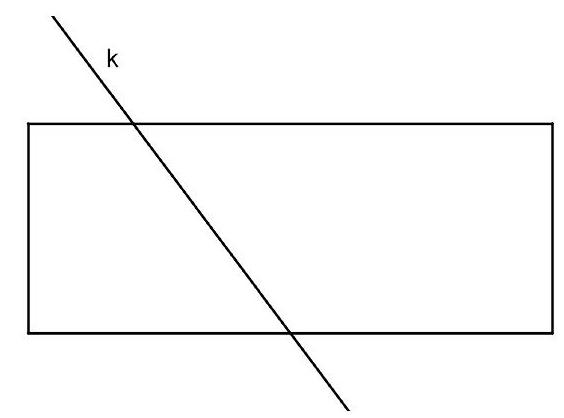
\includegraphics[max width=\textwidth, center]{2024_11_21_51acf29752b622e5581fg-1}


\end{document}